%!TEX root = ../thesis.tex

\begin{savequote}[70mm]
	The Internet is becoming the town square for the global village of tomorrow.
	\qauthor{Bill Gates}
\end{savequote}


\chapter{Technologies}\label{chapter:technologies}
	
	This chapter explains more in detail the underlying technologies of this project.
	Starting from the general definition of a network and the most common architectures, to radio technologies work and then micro-controllers.
	
\section{Fundamentals of network communication}
	
	\begin{center}
		\begin{minipage}[H]{0.9\columnwidth}
			\begin{center}
				``\textit{A computer network is a structure that makes available to a data processing user at one place some data processing function or service performed at another place.}''~\cite{nla.cat-vn252493}
			\end{center}
		\end{minipage}
	\end{center}
	
	Starting from the definition of a computer network by Paul E. Green, it is easy to understand its importance in today's society.
	Smartphones, personal computers and other interconnected devices have become omnipresent in modern society, in which people need to feel connected to each other via these devices.
	% https://www.irishtimes.com/business/online-services-playing-more-important-role-in-everyday-activities-1.511857
	Not only they are used for fun, leisure and other social activities, but they allow connection to services such as online banking, government services and healthcare, that require a stable and secure connection among the systems that they use in order to provide a safe and sound experience for their users.
	All this to say, networks are everywhere underneath today's technology.
	There are no services or devices that can stand on their own without sharing data to other devices, to synchronize and provide a better user experience, to get updates from the manufacturer or simply to send a keep alive message.
	
	While this raw data is important for computers, people, the final users, process it to gain information, and this exchange of information from all around the world has brought radical changes many levels, from a cultural point of view to an economic point of view.
	The possibility of having a network of information exchange is the next step of globalization, which started with the exchange of goods among countries and now brings everyone together, allowing for a cultural exchange that lets people share and unite across the globe.
	
	This big network that is used to exchange information all around the world has a special name: Internet.
	% https://en.wikipedia.org/wiki/Right_to_Internet_access	
	% https://www.diplomacy.edu/blog/right-access-internet-countries-and-laws-proclaim-it/
	Many countries, such as Finland, Spain and Greece, have recognized the importance of this network and have given people the ''right to Internet access'', also known as the right to broadband or freedom to connect
	In these countries, service providers must be able to supply a mandatory minimum connection capability to all desiring home users in the regions of the country they serve.
	
	% http://www.redbooks.ibm.com/abstracts/gg243376.html
	It is important to note that Internet, with a capital I, is a particular set of worldwide interconnected networks \cite{gg243376}, but a common network of networks is called internetwork, shortened by internet, with a lowercase i.
	
	Such distinction began in the 1980s and has been described in RFCs \footnote{\href{https://datatracker.ietf.org/doc/html/rfc871}{RFC 871 (1982): A PERSPECTIVE ON THE ARPANET REFERENCE MODEL}}$^{,}$\footnote{\href{https://datatracker.ietf.org/doc/html/rfc872}{RFC 872 (1982): TCP-ON-A-LAN}} by computer scientists that understood how ARPANET was expanding and the its dimensions were not enough anymore to accommodate the amount of data traveling from one computer to another.
	% https://en.wikipedia.org/wiki/Commodore_64
	At that time, computers such as the IBM 5150 and the infamous Commodore 64 were starting to become more and more available, even if highly priced, not only to companies and universities, but also to consumers that brought them in their households, especially with the advent of MS-DOS, the dominant operating system throughout the 1980s and now open source \footnote{\url{https://github.com/microsoft/MS-DOS}}.
	
	As described by IBM in one of their technical books from the time, ''it is possible to divide the Internet such as the following groups of networks''\cite{gg243376}:
	\begin{itemize}[noitemsep]
		\item Backbones: large and strategical data routes among core networks and routers that compose and connect the Internet;
		\item Regional networks that connect large facilities such as universities and colleges;
		\item Commercial networks that provide to their subscribers access to the Internet;
		\item Local networks which run, for example, across a campus university;
	\end{itemize}

	% TODO sistemare posizione footnote alla fine
	% Oppure prendere mappa da https://www.globalbackbone.tisparkle.com/
	% Mettere riferimento a mappa interattiva
	% https://globe.gl/example/submarine-cables/
	\begin{figure}
		\centering
		\includegraphics[width=\textwidth]{resources/img/chap3/backbone}
		\caption[Subsea Internet backbone cables between US and Europe.]{Subsea Internet backbone cables between US and Europe. \footnotemark}
	\end{figure}
	\footnotetext{~\url{https://www.infrapedia.com/app}}

	Given this increase of computers connecting to the Internet, there came the need for a revised structure that could better organize these components in a more robust, but also flexible, large network.

	With more accessible OSs, such as Windows 95 and Windows 98, and the advent of Tim Berners-Lee's World Wide Web (or WWW), computers became a commodity present in many households.
	The invention of the web and its ease to navigate, using hyperlinks and search engines, culminated in the dot com bubble, a stock market bubble in the late 90s that caused rapid rise of technology companies in stock market.
	
	Networks can be categorized based on the area they cover and serve:
	\begin{itemize}[noitemsep]
		\item Wide Area Network, or WAN: sometimes called long haul networks, provide communication over long distances;
		% https://www.cloudflare.com/learning/network-layer/what-is-a-metropolitan-area-network/
		\item Metropolitan Area Network, or MAN: provide communication inside a metropolitan area, which could be a single large city, multiple cities, or any given large area with multiple buildings;
		\item Local Area Network, or LAN: provide the highest speed connections among computers in a small and circumscribed area;
		% https://www.cloudflare.com/learning/network-layer/what-is-a-personal-area-network/
		\item Personal Ara Network, or PAN: connects devices within a user's immediate area.
	\end{itemize}

	In Sec. \ref{sec:radio_tech}, is described another level of distinction based on the power consumed by the transmission medium.
	
	Since everyone can connect to the Internet and access it's services, there is no need for the average user to understand what happens between his machine and the rest of the network, which means he only sees the information that is displayed to him without knowing where it arrives from or what path it took to arrive on his monitor.
	
	% inserire immagine con la nuvoletta che si vede dentro e non si vede dentro ?
	
	For computer scientists though, it is important to understand the difference between network architecture and network topology.	
	A network architecture, as described by by Paul E. Green, ``is a complete definition of all the layers necessary to build the network''\cite{nla.cat-vn252493}.
	This is focused on the network software, which needs to be highly structure in order to allow for heterogeneous systems to communicate with each other.
	% https://standards.iso.org/ittf/PubliclyAvailableStandards/s020269_ISO_IEC_7498-1_1994(E).zip
	One example of network architecture is the ISO/OSI reference model \footnote{\url{https://www.iso.org/standard/20269.html}}, which is implemented by the TCP/IP stack of protocols.
	
	% https://stackoverflow.com/questions/38596488/in-which-layer-is-http-in-the-osi-model
	\begin{figure}[H]
		\centering
		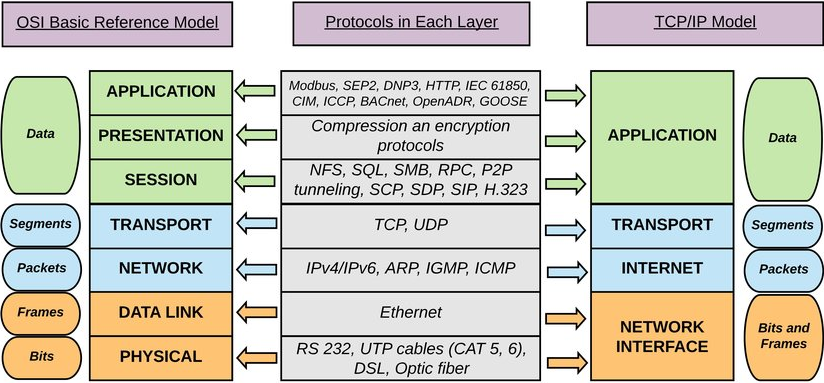
\includegraphics[width=\textwidth]{resources/img/chap3/isoosi}
		\caption{The ISO/OSI reference model against the TCP/IP stack}
	\end{figure}
	
	Thus comes the definition of a protocol as ``a set of agreements for interaction of two or more parties and is expressed by three components, syntax (e.g., a set of headers, a set of commands/responses), semantics (the actions and reactions that take place, including the exchange of messages), and timing, the sequencing and concurrency aspects of the protocol.''\cite{nla.cat-vn252493}.
	% TODO rivedere contenuto tra parentesi
	Different types of network use different architectures, based on the transmission medium and how well this performs (errors, speed, etc.).
	
	% https://www.omnisci.com/technical-glossary/network-topology
	On the other hand, the network topology refers to the manner in which the links and nodes of a network are arranged to relate to each other.
	
	\begin{figure}[H]
		\centering
		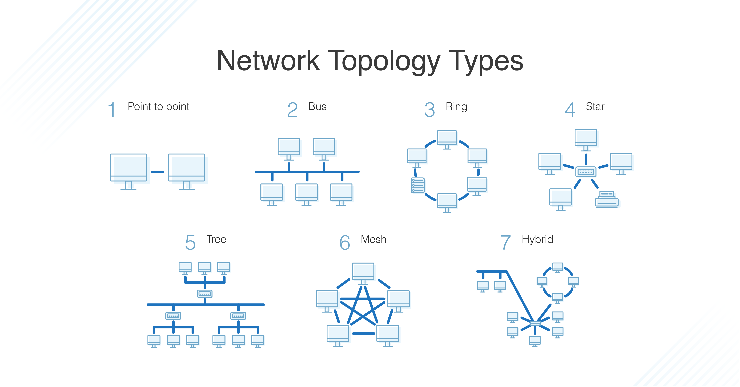
\includegraphics[width=\textwidth]{resources/img/chap3/network_topologies.png}
		\caption{Common network topologies}
		\label{img:network_topologies}
	\end{figure}
	
	As shown in Fig. \ref{img:network_topologies}, some of the most common network topologies are:
	\begin{itemize}[noitemsep]
		\item Point-to-Point: in which devices are connected directly;
		\item Bus: devices are connected to each other via a backbone cable;
		\item Ring: two dedicated point-to-point links connect a device to the two devices located on either side of it, creating a ring of devices through which data is forwarded via repeaters until it reaches the target device;
		\item Star: connects each device in the network to a central hub. Devices can only communicate with each other indirectly through the central hub;
		\item Tree: parent-child hierarchy in which star networks are interconnected via bus networks;
		\item Mesh: a dedicated point-to-point link connects each device on the network to another device on the network, only carrying data between two device;
		\item Hybrid: any combination of two or more topologies;
	\end{itemize}

	% TODO rivedere bene quando si scrive resto della tesi
	The project presented in this thesis regards a network with a mesh topology.
	This is better described in chap5 in a more depth and technical way
	The mesh proposed in this thesis has a span of LAN / MAN, since it connects devices that are in a circumscribed area but can be also placed further from each other, in order to cover longer distances.
	
	% TODO è necessaria?
	Another important distinction to make is the one between a distributed systems and a computer network.
	
	% COPIATO DA INTERNET: responsible for technical management of IETF activities and the Internet standards process
	Nowadays, the organization responsible for technical management of IETF activities and the Internet standards process is the Internet Engineering Steering Group (IESG)\footnote{\url{https://www.ietf.org/about/groups/iesg/}}.
	It is necessary to have an organization looking over the Internet itself since it gives the regulations that allow all devices to interconnect with each other.

\section{Radio technologies}\label{sec:radio_tech}
	
	% https://en.wikipedia.org/wiki/Invention_of_radio
	Although Guglielmo Marconi is usually credited as the inventor of radio due, to the creation of the first commercially successful wireless communication system \cite{4137304}, many scientists before him have studied the subject of radio waves.
	The discovery of electromagnetic waves, including radio waves, by Heinrich Rudolf Hertz in the 1880s, came after theoretical development on the connection between electricity and magnetism that started in the early 1800s.
	Scientists tried to achieve the idea of a wireless telegraph via electric conduction and electromagnetic induction for a while before the establishment of radio-based communication.
	
	% https://science.howstuffworks.com/innovation/inventions/who-invented-the-radio.htm
	Other important experiments were made by Nikola Tesla, who invented the Tesla coil, a device essential to sending and receiving radio waves, during efforts to develop a "wireless" lighting system.
	% TODO aggiungere patent?
	This Tesla coil has been used by Marconi in his experiments and is present in the patent he presented for radio transmission of data.
	
	More than a century later, radio technology has massively evolved and is used on a daily basis.
	Devices has shrunk and the amount of transmission meanings have increased far from what both Tesla and Marconi could have thought of.
	Thus, in order to give a complete picture of radio transmitting technologies, it is important to make a distinction among the ones that are made for internal or nearby use vs the ones that are used for longer distances.
	
	% https://sites.google.com/site/pnutpck11/lesson-9---wireless-transmission-media
	Many users opt for wireless transmission media because it is more convenient than installing cables, even if they might sacrifice some performance. 
	Also, using wireless technology allows transmission in locations where it is impossible to install cables.
	% TODO RIVEDERE COPIATA SPUDORATAMENTE
	Types of wireless transmission media used in communications include infrared, broadcast radio, cellular radio, microwaves, and communications satellites.
	\begin{itemize}[noitemsep]
		\item Infrared: wireless transmission medium that sends signals using infrared light waves
		\item Broadcast Radio: wireless transmission medium that distributes radio signals through the air over long distances such as between cities, regions, and countries and short distances such as within an office or home. Bluetooth, UWB, Wi-Fi, and WiMAX communications technologies use broadcast radio signals.
		\item Cellular Radio: form of broadcast radio that is used widely for mobile communications, specifically wireless modems and cell phones, which use high-frequency radio waves to transmit voice and digital data messages.
		\item Communications satellite: space station that receives microwave signals from an earth-based station, amplifies (strengthens) the signals, and broadcasts the signals back over a wide area to any number of earth-based stations.
		Applications such as air navigation, television and radio broadcasts, weather forecasting, video conferencing, paging, global positioning systems, and Internet connections use communications satellites.
	\end{itemize}
	
	With new transmission technologies, new network architectures and topologies that are better suited for the transmission method have emerged.
	Topologies that bring computation closer to the edge are also rising in popularity, since they allow for faster computation and they bring data closer to the user.
	
	LAN MAN and WAN are not enough anymore to describe the new topologies.
	An important distinction is now made by other factors such as power consumption, cost of the devices and range of the transmiter and receiver.
	
	The most important new category of wireless communication, that interests IoT and reprents a large portion of the market at the time of writing, as described in chap2, is LPWAN, which stands for Low Power Wide Area Networks.
	
	The characteristics of LPWAN are: long range, low power and low cost.
	% https://en.wikipedia.org/wiki/Low-power_wide-area_network
	Lightweight protocols reduce complexity in hardware design and lower device costs. Its long range combined with a star topology reduce expensive infrastructure requirements, and the use of license-free or licensed bands reduce network costs.

	% http://iotfactory.eu/iot-knowledge-center/overview-of-iot-networks/	
	% TODO CAMBIARE E CITARE
	% https://www.mdpi.com/1999-5903/12/3/46
	The growing popularity of IoT use cases in domains that rely on connectivity spanning large areas and the ability to handle a massive number of connections is driving the demand for LPWAN access technologies \cite{fi12030046}, and the project presented in this thesis falls under this category of communication.
	LPWAN allows connectivity in many applications, from crowded areas in smart cities to smart farming and smart environment, from security and emergencies to e-health.
	
	Various wireless transmission methods can be used to create a LPWAN, some of the most used in IoT are Sigfox, LoRa and NarrowBand IoT (NB-IoT).
	In subsection \ref{subsec:lora_lorawan}, follows a more complete explanation on LoRa and LoRaWAN.
	One important factor for all these transmission methods is to support a massive number of simultaneously connected devices with low data rates \cite{fi12030046}.
	
	Other important communication technologies in IoT are RFID, NFC, for contact purposes, Bluetooth, Zigbee for a personal network and IEEE 802.11, or WiFi, for a local area.
	The latter was used in the ArduEco project, described in chap2.
	Fig. \ref{img:wireless_coverage} contains a representation of the geographic coverage in meters of the various aforementioned wireless transmission methods.

	
	% TODO sistemare posizionamento immagine
	% \newpage
	\begin{figure}
		\centering
		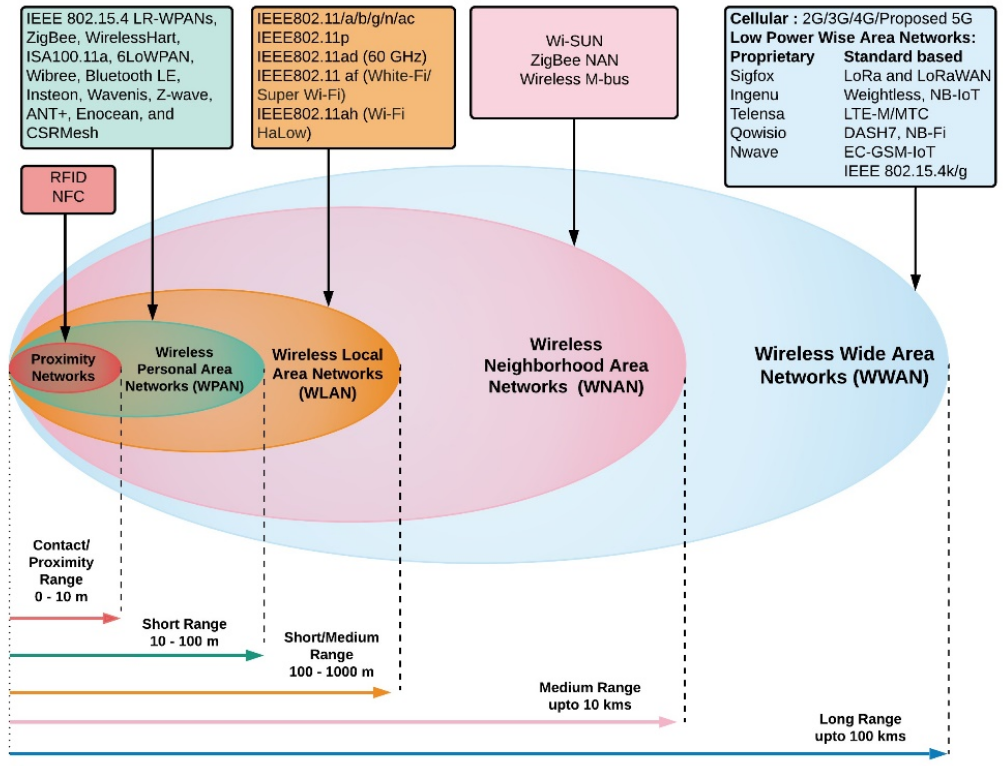
\includegraphics[width=\textheight,height=\textwidth,keepaspectratio,angle=90]{resources/img/iot_range}
		% 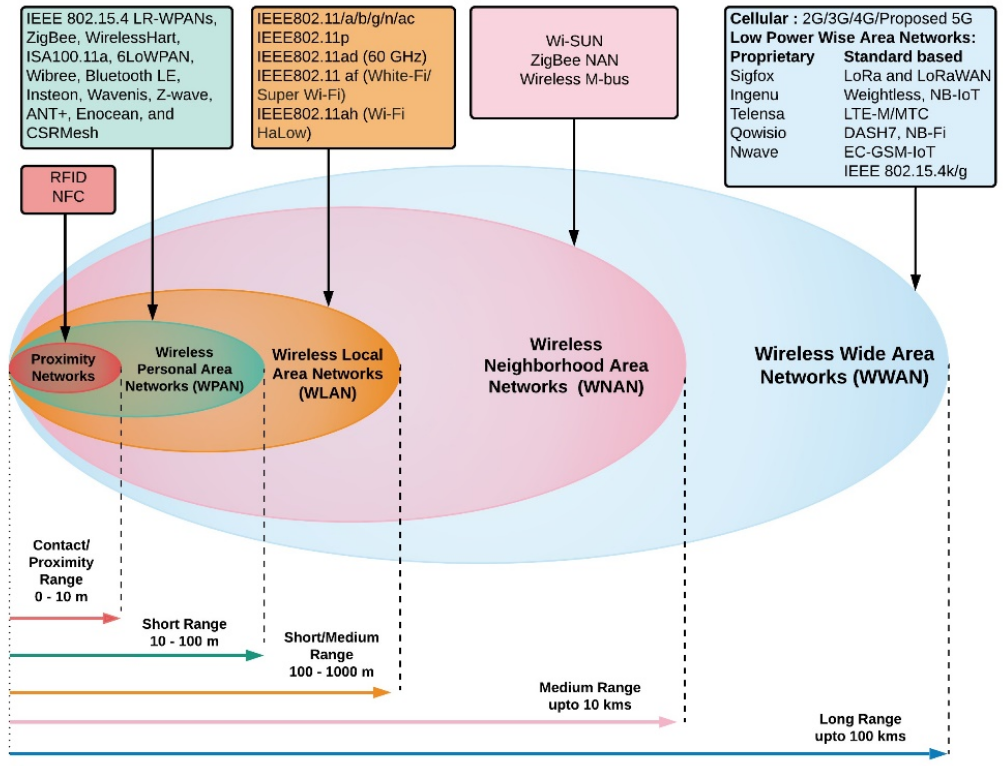
\includegraphics[height=\textwidth, angle=90]{resources/img/iot_range}
		\caption[Wireless access geographic coverage.]{Wireless access geographic coverage. \cite{fi12030046}}
		\label{img:wireless_coverage}
	\end{figure}
	% \newpage

	\subsection{LoRa and LoRaWAN}\label{subsec:lora_lorawan}
	
		% TODO modificare perchè copiato spudoratamente
		% https://www.semtech.com/lora
		LoRa (short for long range) is a spread spectrum modulation technique derived from chirp spread spectrum (CSS) technology.
		Semtech’s LoRa is a long range, low power wireless platform that has become the de facto wireless platform of Internet of Things (IoT).
		
		% https://www.design-reuse.com/news/28706/semtech-cycleo-acquisition.html
		% https://blog.semtech.com/a-brief-history-of-lora-three-inventors-share-their-personal-story-at-the-things-conference
		Since it's development in 2009, by the french company Cycleo, now acquired by the semiconductor company Semtech, LoRa has come a long way.				
		On top of it, there is a proprietary MAC protocol called “LoRaMAC”, which specifies the message formats and security layers for a true networking protocol.
		
		In February 2015, the LoRa Alliance was founded and the networking protocol was renamed “LoRaWAN.”
		% https://lora-alliance.org/
		The LoRa Alliance is a non-profit organization committed to enabling large-scale deployment of Low Power Wide Area Networks (LPWAN) IoT through the development and promotion of the LoRaWAN open standard.
		
		This organization is alike with the 3GPP 
		
		Applications of LoRa in IoT varies from smart agriculture, to smart cities, to contact tracing, to logistics and healthcare.
		A complete list of the whitepapers on LoRa based communication can be found on Semtech's official website \footnote{\url{https://www.semtech.com/lora/lora-applications}}.
		
		% TODO aggiungere tabella con specifiche
		
		\begin{figure}[H]
			\centering
			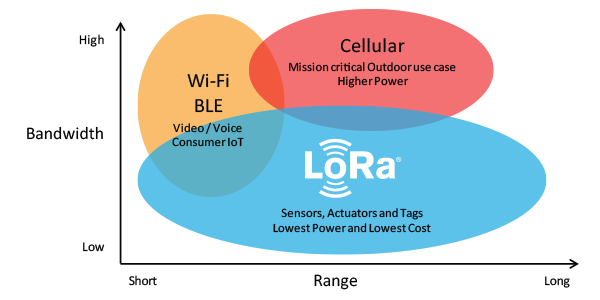
\includegraphics[width=\textwidth]{resources/img/LoRa_Why_Range}
			\caption{}
		\end{figure}

%		The smaller the package, the greater the range.
%		The greater the range, the fewer receiving antennas.
%		The fewer antennas, the lower the total costs for the user.

\section{Hardware (Microcontrollers)}\label{sec:microcontrollers}

	Microcontrollers (or MCUs, short for Microcontroller Unit) are compact integrated circuits designed to govern a specific operation in an embedded system.
	They are specially made to fit in particular environments or to perform specific functions, which usually do not require any particular computation, memory capacity or power.
	This has been made possible thanks to the continuous shrinking of transistors, which makes almost all the components more compact, and the improved power sources.
	% TODO cambiare batteries con qualcos'altro?
	In junction with the previously described wireless technologies, microcontrollers are at the hearth of IoT devices, described in Chap. \ref{chap:background}, and they require long-lasting, low-cost, and sustainable batteries.
	
	% TODO modificare un attimo
	% TODO da riprendere in chap2
	% https://ieeexplore.ieee.org/abstract/document/9148855?casa_token=ppFhpgagThgAAAAA:u81u3jhRB-EJxsnQFx32i8LI4nJBKi3NsDvemcunZKNeSETGloW8wRB45S5OeaYOOdh2kXQ
	The number of IoT connected devices is expected to grow up to 75 billion worldwide by 2025 \cite{statista}, and connection density is expected to be one million devices per square km\cite{noma}.
	These devices will generate massive data and consume significant energy.
	
	Given the amount of specific functions an MCU can perform, there are many boards on the market.
	Some are very alike, while others are very different, since they are expected to be used in other types of environments.
	All boards consist on a similar architecture, which contains the processing unit (CPU), along with memory and programmable input/output peripherals.
	
	\begin{figure}[H]
		\centering
		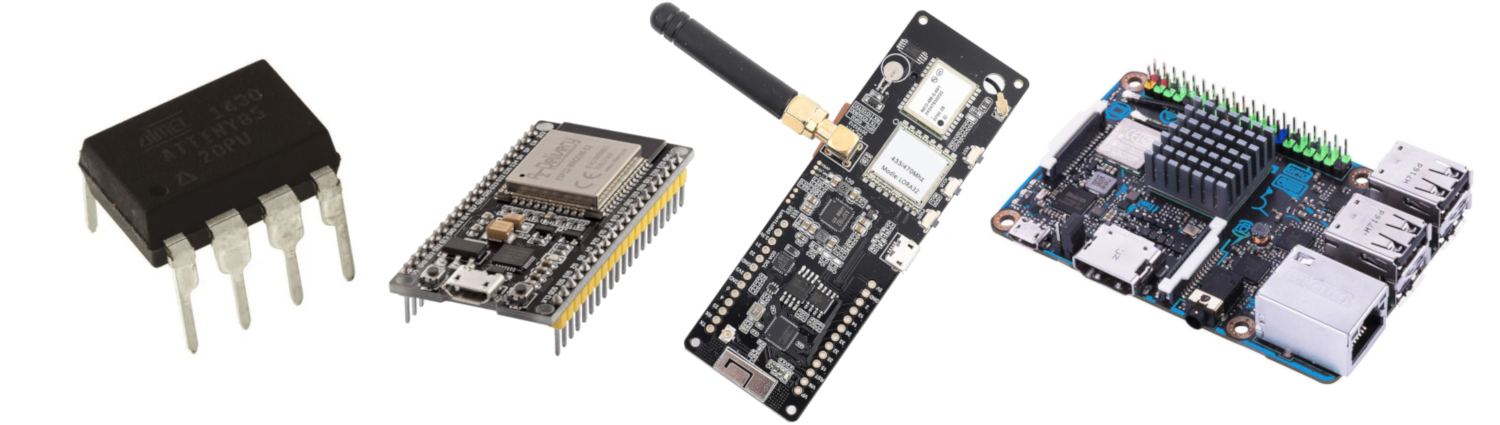
\includegraphics[width=\textwidth]{resources/img/chap3/generic_board}
		\caption{Attiny 85 on the left, in the middle two boards based on the ESP32, on the right the Asus Tinkerboard 2}
		\label{img:generic_board}
	\end{figure}

	% https://en.wikipedia.org/wiki/Microcontroller
	In Fig. \ref{img:generic_board}, there are four different boards, the one farthest on the left is the ATtiny 85 \footnote{\url{https://www.microchip.com/en-us/product/ATTINY85}}, a low-power, 8-bit microcontroller that is made for general purpose and can be programmed for simple tasks, from simple LEDs flashing, to more elaborate small sensor projects.
	% https://en.wikipedia.org/wiki/ESP32
	The two boards in the middle are based on the ESP32 chip, a series of low-cost, low-power system on a chip microcontrollers with integrated Wi-Fi and dual-mode Bluetooth.
	They both are more powerful than the ATtiny 85, and right one offers an integrated LoRa antenna on board.
	Far on the right, there is the Asus Tinkerboard 2 \footnote{\url{https://tinker-board.asus.com/product/tinker-board-2.html}}, a board powered by an Arm 6-core system on a chip (SoC), with a 64-bit Armv8 architecture.
	This board provides much more computing power compared to the previous ones and is able to run operating systems such as Linux and Windows.
	
	% https://www.amazon.it/Meipai-ATTINY85-20PU-ATTINY85-chip-ATMEL/dp/B08HPPMJ52/
	% https://www.amazon.it/AZDelivery-NodeMCU-Development-Arduino-gratuito/dp/B071P98VTG/
	% https://www.amazon.it/Scheda-Modulo-Wireless-T-Beam-Batteria/dp/B07X2KPN4L/
	% https://www.welectron.com/navi.php?qs=Tinker
	One of the strong points of these boards is the price: the ATtiny is priced around 1€ when bought in bulk, the boards on the middle cost around 7€ and 15€, while the board by Asus is the more expensive and starts from 70€.
	
	It is important to note though that using a generic board in a production environment might not be ideal, since it might lack of support and documentation.
	The boards described subsequently are from three of the major MCU producers, Arduino, Raspberry Pi and Pycom, which have built hardware that is well documented and suited for many different environments, from hobbysts to industrial use.
	
	The simplified architectures and the constraints of embedded devices are reflected in the narrow choice for programming languages.
	It is hard to find an MCU programmed in Java since this would require the JVM running in the background.
	Popular languages for MCUs are, for example, C/C++, Assembly, Rust, Ada, Erlang, etc.
	% TODO CONTROLLARE
	All these have in common the fact that they are compiled and the bytecode has a small footprint.
	A particular microcontroller company, Arduino, have developed a version of C++ specific for their boards, but given the simplictity of this new dialect, many boards on the market can be programmed with it.
	Arduino is explained further in Subsection \ref{subsec:arduino}.

	% TODO da spostare in 
	Another programming language that is quickly taking hold at the time of writing, is Mycropython.
	As explained in their website it is an "efficient implementation of the Python 3 programming language that includes a small subset of the Python standard library and is optimised to run on microcontrollers and in constrained environments" \footnote{\url{https://micropython.org/}}.
	% https://itqna.net/questions/437/what-definition-verbose-code-and-why-it-interesting-reduce-i
	Python's fast learning and explicit code advantages are reflected in this smaller version for microcontrollers, available for most of them.
	
	Below is a table with the specifications of microcontrollers from Arduino, Raspberry Pi and Pycom, which are better described in the following subsections.
	\begin{table}[htbp]
		\begin{center}
			\begin{tabularx}{\textwidth}{@{}|Y|Y|Y|Y|Y|Y|@{}} 
				\hline
				& Arduino UNO R3 & Arduino Nano BLE & Raspberry Pi & Rasperry Pi Pico & Pycom FyPy \\\hline
					CPU &&&&& \\\hline
					RAM &&&&& \\\hline
					ROM &&&&& \\\hline
					IO PINS &&&&& \\\hline
					PORTS &&&&& \\\hline
			\end{tabularx}
			\caption{Specifications of Arduino, Raspberry Pi and Pycom microcontrollers}
			\label{table:1}
		\end{center}
	\end{table}

	\subsection{Arduino}\label{subsec:arduino}
	
		% https://www.arduino.cc/en/Main/AboutUs
		% https://www.oreilly.com/library/view/arduino-a-technical/9781491934319/ch01.html	
		Arduino is a company founded by Massimo Banzi Et Al. in Ivrea, Italy, in 2005, and has released the first commercially available microcontroller.
		% TODO rivedere
		They wanted a device that was simple, easy to connect to various ''things'' (such as relays, motors, and sensors), and easy to program, besides being inexpensive.
		% It also needed to be inexpensive, as students and artists aren’t known for having lots of spare cash. 
	
		They selected the AVR family of 8-bit microcontroller devices from Atmel and designed a self-contained circuit board with easy-to-use connections, wrote bootloader firmware for the microcontroller, and packaged it all into a simple integrated development environment (IDE) that used programs called “sketches”. 
		Arduino was the result.
		
		The most famous version of their board is the UNO (one in English).
		Arduino UNO, the one on the left in Fig. \ref{img:arduino_board}, is the most used and documented board of the whole Arduino family.
		% https://www.circuito.io/blog/arduino-uno-pinout/
		Although this board does not have any integrated sensors or particular ports for peripherals.
		The current revision of the board is the Arduino UNO Rev 3 \footnote{\url{https://store.arduino.cc/products/arduino-uno-rev3}}, which consists of 14 digital pins, 6 analog inputs, a power jack, USB connection and ICSP header.
		
		% https://store.arduino.cc/products/arduino-uno-rev3
		% https://store.arduino.cc/products/arduino-yun-rev-2
		% https://store.arduino.cc/products/arduino-nano-33-ble
		\begin{figure}[H]
			\centering
			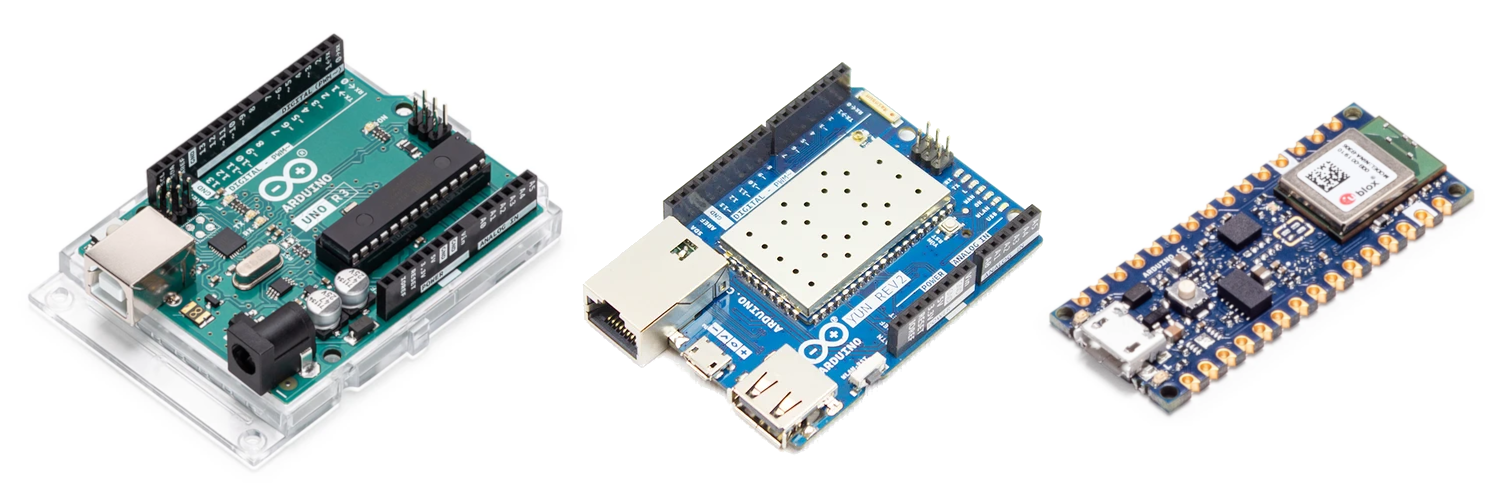
\includegraphics[width=\textwidth]{resources/img/chap3/arduino_types}
			% TODO rivedere accento yun, mettere link?
			\caption{Arduino UNO Rev 3 on the left, Arduino Yun in the middle, Arduino Nano 33 BLE on the right}
			\label{img:arduino_board}
		\end{figure}
		
		% https://www.circuito.io/blog/arduino-code/
		The Arduino family of products can be programmed in a particular programming language based on C/C++, using a special open-source integrated development environment (IDE).
		Arduino was so disruptive in the market that many boards, included the ones in Fig. \ref{img:generic_board}, support the Arduino C++.

		Shields are modular circuit boards that can be added to extend capabilities to different application needs.
		These can be attached directly on top of the board and provide sensors, interfaces, peripherals on a single board, rather than attaching to the Arduino singularly.
		% https://learn.sparkfun.com/tutorials/arduino-shields
		Some of the functionalities that can be added by a shield are Ethernet, WiFi, GPS, displays and cameras, motor drivers.
		Most of the additional shields on the market have been developed for the Arduino UNO, since it is the most common board.
		
		The choice of making the Arduino schematics open-source and accessible to anyone has largely favored the development of newer boards, similar in capacity to the Arduino but more specialized, since producers and board makers are able to keep only the components needed or add different ones.
		An example can be the two middle boards in Fig. \ref{img:generic_board}, which rode the wave of Arduino's popularity.
		Not only the datasheets are available for all boards, but also the Arduino IDE software is open-source.
		
		% https://www.circuito.io/blog/arduino-code/
		The versatility of Arduino and its simple interface makes it a leading choice for a wide range of users around the world from hobbyists, designers, and artists to product prototypes. 
		
		Newer Arduino boards offer many integrated functionalities, for example:
		\begin{itemize}[noitemsep]
			% https://store.arduino.cc/collections/boards/products/arduino-mkr-nb-1500
			\item Arduino MKR NB 1500: offers an all-in-one solution for Narrowband IoT large-coverage solutions;
			% https://store.arduino.cc/collections/boards/products/arduino-mkr-wifi-1010
			\item Arduino MKR WiFi 1010: offers integrated WiFi and Bluetooth;
			% https://store.arduino.cc/collections/boards/products/arduino-nano-33-ble-sense
			\item Arduino Nano 33 BLE Sense: contains BLE connectivity and multiple sensors, such as 9 axis inertial, humidity, and temperature, barometric, microphone, gesture, proximity, light color and light intensity.
		\end{itemize}
	
		% TODO rivedere bene quando si scrive resto della tesi
		Particularly, this last model, the board on the right in Fig. \ref{img:arduino_board}, has been considered as one of the possible choices as development board for this project.
		As better explained in chap 5, it has been discarded since it does not offer LoRa connectivity and an additional module would have been necessary to connect the board in a mesh.
							
	\subsection{Raspberry Pi}

		% https://ccclib.org/raspberrypi/
		% https://www.electronicshub.org/raspberry-pi-vs-arduino/
		Another important microcontroller on the market is the Raspberry Pi, developed by Eben Upton at the University of Cambridge in the United Kingdom with the aim of teaching and improving programming skills of students in developing countries.
		
		Compared to the Arduino specifications, it also offers more functionalities, since they include an ARM processor, a GPU with HDMI output connectivity, an Ethernet port, USB ports to connect mouse and keyboard, a camera interface, more RAM memory and more I/O pins.
		% https://www.makeuseof.com/tag/what-is-an-arm-processor/
		ARM processors, or Advanced RISC Machine processors, are better suited to mobile computing, since they use a simplified, less power-hungry method of processing.
		This allows the Raspberry Pi to run full operating systems such as some Linux distributions, included the official operating system Raspian OS
		
		% TODO rivedere perchè copiato
		Since the entire Computer (the Processor, RAM, Storage, Graphics, Connectors, etc.) is sitting on a single Printed Circuit Board, the Raspberry Pi (and other similar boards) are called as Single Board Computers or SBC.
		
		Letting their differences aside, both are very popular boards among electronics DIY builders, hobbyists and even professionals.
		Some projects involve the use of both boards in a master-slave architecture, where the Raspberry Pi acts as a master and gathers the data from the Arduinos, which are equipped with the sensors.
		
		Some of the main competitors of the Raspberry Pi are the Banana Pi and the Asus Tinkerboard (in Fig. \ref{img:generic_board}).
		Since, like the Arduino, the Raspberry Pi boards schematics are open-source and available online \footnote{\url{https://www.raspberrypi.org/documentation/computers/raspberry-pi.html}}, board makers have been able to adapt them in their own way.

		% https://en.wikipedia.org/wiki/Raspberry_Pi
		% https://www.raspberrypi.org/products/raspberry-pi-3-model-b-plus/
		
		\begin{figure}[H]
			\centering
			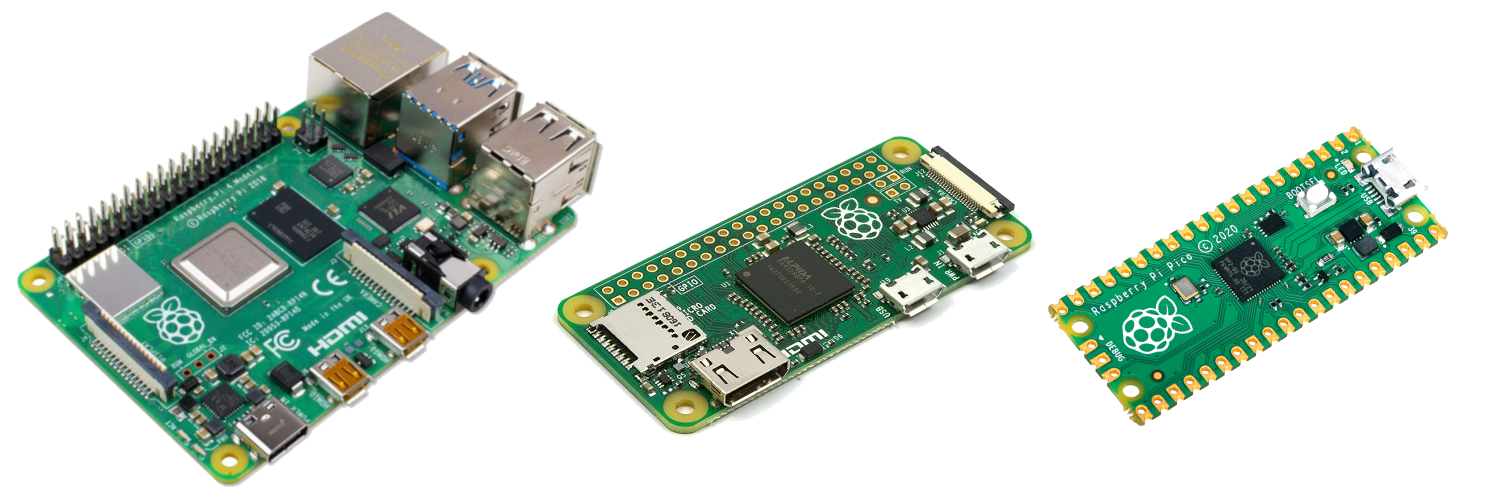
\includegraphics[width=\textwidth]{resources/img/chap3/raspberry_types}
			\caption{Raspberry Pi Model 3B+ on the left, Raspberry Pi Zero in the middle, Raspberry Pi Pico on the right}
			\label{img:raspberry_board}
		\end{figure}
		
		There are now different Raspberry Pi boards, or models, each a bit more specialized than the other.
		Some of the most important models are:
		\begin{itemize}[noitemsep]
			\item 3 B+ / 4: the model 3B+ and 4 are their most selling products, they are marketed as a ''tiny, dual-display, desktop computer'' \footnote{\url{https://www.raspberrypi.org/products/raspberry-pi-4-model-b/}};
			\item Zero: it's the smallest form factor Raspberry Pi on the market;
			\item Pico: a low-cost, high-performance microcontroller board with flexible digital interfaces.
		\end{itemize}
		
		% TODO rivedere prezzi
		They are represented in Fig. \ref{img:raspberry_board} and can be considered as the latest evolution of what is needed to learn programming in a Unix like environment at a low cost, in fact these boards cost 35\$, 5\$ and 3\$ each.
		A complete list of the available boards can be found on their online store \footnote{\url{https://www.raspberrypi.org/products/}}.
		
		% TODO rivedere bene quando si scrive resto della tesi
		The Raspberry Pi Pico was considered for this project, but was rejected since, as the Arduino, it would have needed additional modules for LoRa and BLE connectivity, while the other models have a computational power much greater than the one needed.
			
	\subsection{Pycom}
		
		% https://pycom.io/the-story-of-pycom-things/
		While Raspberry Pi and Arduino share a longer history, Pycom was founded in 2015 via a crowdfunding campaign on Kickstarter with the goal to create a new board for immediate development in the world of IoT, with all the possible connectivity.
		As the other two previously described companies, Pycom offers multiple board choices, such as the fipy, represented in Fig. \ref{img:pycom_board}, the wipy and the lopy.
		These boards are very similar to each other, since all of them offer at least WiFi and BLE, have the same chipset, interfaces and memory.
		
		\begin{figure}[H]
			\centering
			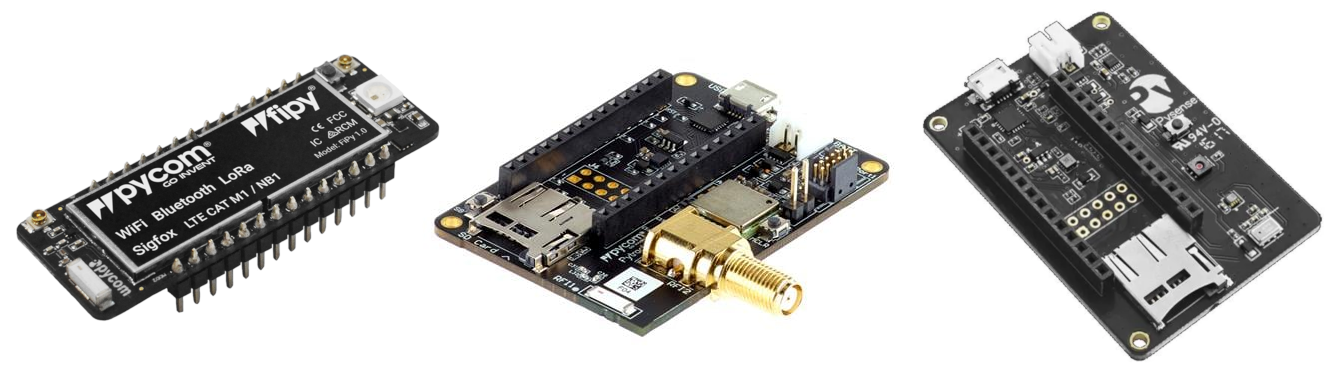
\includegraphics[width=\textwidth]{resources/img/chap3/pycom_board}
			\caption{fypy on the left, PyTrack 2X in the middle, pysense on the right}
			\label{img:pycom_board}
		\end{figure}	
		
		In particular, the FiPy board, has been chosen for this project since it packs five networks in one small board.
		As described in the product page \footnote{\url{https://pycom.io/product/fipy/}}, it is capable to communicate via WiFi, Bluetooth, LoRa, Sigfox and dual LTE-M (CAT-M1 and NB-IoT), and gives access to global LPWAN networks.
		% share similar specifications
		All the boards offered by pycom at the time of writing are equipped with an Espressif ESP32 chipset, 4MB of RAM and an flash memory of 8MB.
		
		% TODO VERIFICARE 
		% https://pycom.io/products/software/open-source/
		% https://eu.mouser.com/manufacturer/pycom/
		Contrary to Arduino and Raspberry Pi, the Pycom has decided to maintain the datasheets and the firmware of their boards proprietary, which means there is far less support from the community when comes to finding bugs in the software or improving the component placement on the board.
		Nonetheless, Pycom boards are chosen for the affability of the company producing them, also because of their high density of hardware on a board with a small footprint.
		
		Additional sensors and functions can be added to Pycom boards via shields, just like the Arduino.
		% https://pycom.io/product/pysense-2-0-x/
		% https://pycom.io/product/pytrack-2-0-x/
		Particularly for this project, the fipy has been integrated with the Pytrack 2x, which add accelerometer and GPS, and the pysense, which add ambient light, pressure and humidity.
		Both expansion boards are represented in Fig. \ref{img:pycom_board}.
				
		% https://docs.pycom.io/pybytes/
		As for the programming language, Pycom boards can be programmed using Mycropython via their Pymakr suite of IDE plugins, the Pymate mobile app, and Pybytes an online middleware platform and desktop application to remotely manage the boards.
		
		About the cost of the boards, the price of the single major components used for this project are, at the time of writing:
		\begin{itemize}[noitemsep]
			% https://pycom.io/product/fipy/
			\item FiPy €59.40
			% https://pycom.io/product/pytrack-2-0-x/
			\item Pytrack 2.0 X €40.65
			% https://pycom.io/product/pysense-2-0-x/
			\item Pysense €29.65
		\end{itemize}
		
		Although higher than an Arduino board, it is important to consider that these boards offer and all in one solution.
		The additional cost in buying an external generic shield for an Arduino board would be reflected not only on the money spent on the shield itself, but also in the time and effort of configuring and troubleshooting it in case of errors.
		An overall advantage of Pycom's products is the tight ecosystem, which allows for faster and easier troubleshooting, configuration and programming.
		All these factors are well described in Pycom's documentation on their website \footnote{\url{https://docs.pycom.io/}}.
		
		% TODO rivedere bene quando si scrive resto della tesi
		A more in depth description of how the chosen technologies interact is present in chap5.	